%%%%%%%%%%%%%%%%%%%%%%%%%%%%%%%%%%%%%%%%%%%%%%%%%%%%%%%%%%%%%%%%%%%%%%
% LaTeX Template: Curriculum Vitae
%
% Source: http://www.howtotex.com/
% Feel free to distribute this template, but please keep the
% referal to HowToTeX.com.
% Date: July 2011
% 
%%%%%%%%%%%%%%%%%%%%%%%%%%%%%%%%%%%%%%%%%%%%%%%%%%%%%%%%%%%%%%%%%%%%%%
% How to use writeLaTeX: 
%
% You edit the source code here on the left, and the preview on the
% right shows you the result within a few seconds.
%
% Bookmark this page and share the URL with your co-authors. They can
% edit at the same time!
%
% You can upload figures, bibliographies, custom classes and
% styles using the files menu.
%
% If you're new to LaTeX, the wikibook is a great place to start:
% http://en.wikibooks.org/wiki/LaTeX
%
%%%%%%%%%%%%%%%%%%%%%%%%%%%%%%%%%%%%%%%%%%%%%%%%%%%%%%%%%%%%%%%%%%%%%%
\documentclass[paper=a4,fontsize=11pt]{scrartcl} % KOMA-article class
							
\usepackage[norsk]{babel}
\usepackage[utf8x]{inputenc}
\usepackage[protrusion=true,expansion=true]{microtype}
\usepackage{amsmath,amsfonts,amsthm}     % Math packages
\usepackage{graphicx}                    % Enable pdflatex
%\graphicspath{ {./images/} }
\usepackage[svgnames]{xcolor}            % Colors by their 'svgnames'
\usepackage{geometry}
	\textheight=700px                    % Saving trees ;-)
\usepackage{url}
\frenchspacing              % Better looking spacings after periods
\pagestyle{empty}           % No pagenumbers/headers/footers

%%% Custom sectioning (sectsty package)
%%% ------------------------------------------------------------
\usepackage{sectsty}

\sectionfont{%			            % Change font of \section command
	\usefont{OT1}{phv}{b}{n}%		% bch-b-n: CharterBT-Bold font
	\sectionrule{0pt}{0pt}{-5pt}{3pt}}

%%% Macros
%%% ------------------------------------------------------------
\newlength{\spacebox}
\settowidth{\spacebox}{8888888888}			% Box to align text
\newcommand{\sepspace}{\vspace*{1em}}		% Vertical space macro

\newcommand{\MyName}[1]{ % Name
		\Huge \usefont{OT1}{phv}{b}{n} \hfill #1
		\par \normalsize \normalfont}
		
\newcommand{\MySlogan}[1]{ % Slogan (optional)
		\large \usefont{OT1}{phv}{m}{n}\hfill \textit{#1}
		\par \normalsize \normalfont}

\newcommand{\NewPart}[1]{\section*{\uppercase{#1}}}

\newcommand{\PersonalEntry}[2]{
		\noindent\hangindent=2em\hangafter=0 % Indentation
		\parbox{\spacebox}{        % Box to align text
		\textit{#1}}		       % Entry name (birth, address, etc.)
		\hspace{1.5em} #2 \par}    % Entry value

\newcommand{\SkillsEntry}[2]{      % Same as \PersonalEntry
		\noindent\hangindent=2em\hangafter=0 % Indentation
		\parbox{\spacebox}{        % Box to align text
		\textit{#1}}			   % Entry name (birth, address, etc.)
		\hspace{1.5em} #2 \par}    % Entry value	
		
\newcommand{\EducationEntry}[4]{
		\noindent \textbf{#1} \hfill      % Study
		\colorbox{Black}{%
			\parbox{6em}{%
			\hfill\color{White}#2}} \par  % Duration
		\noindent \textit{#3} \par        % School
		\noindent\hangindent=2em\hangafter=0 \small #4 % Description
		\normalsize \par}

\newcommand{\WorkEntry}[4]{				  % Same as \EducationEntry
		\noindent \textbf{#1} \hfill      % Jobname
		\colorbox{Black}{\color{White}#2} \par  % Duration
		\noindent \textit{#3} \par              % Company
		\noindent\hangindent=2em\hangafter=0 \small #4 % Description
		\normalsize \par}

\newcommand{\Test}[4]{
		\noindent \textbf{#1} \hfill      % Study
		\colorbox{Black}{%
			\parbox{6em}{%
			\hfill\color{White}#2}} \par  % Duration
		\noindent \textit{#3} \par        % School
		\noindent\hangindent=2em\hangafter=0 \small #4 % Description
		\normalsize \par}

%%% Begin Document
%%% ------------------------------------------------------------
\begin{document}
 %you can upload a photo and include it here...
%\begin{wrapfigure}{l}{0.5\textwidth}
	%\vspace*{-2em}
		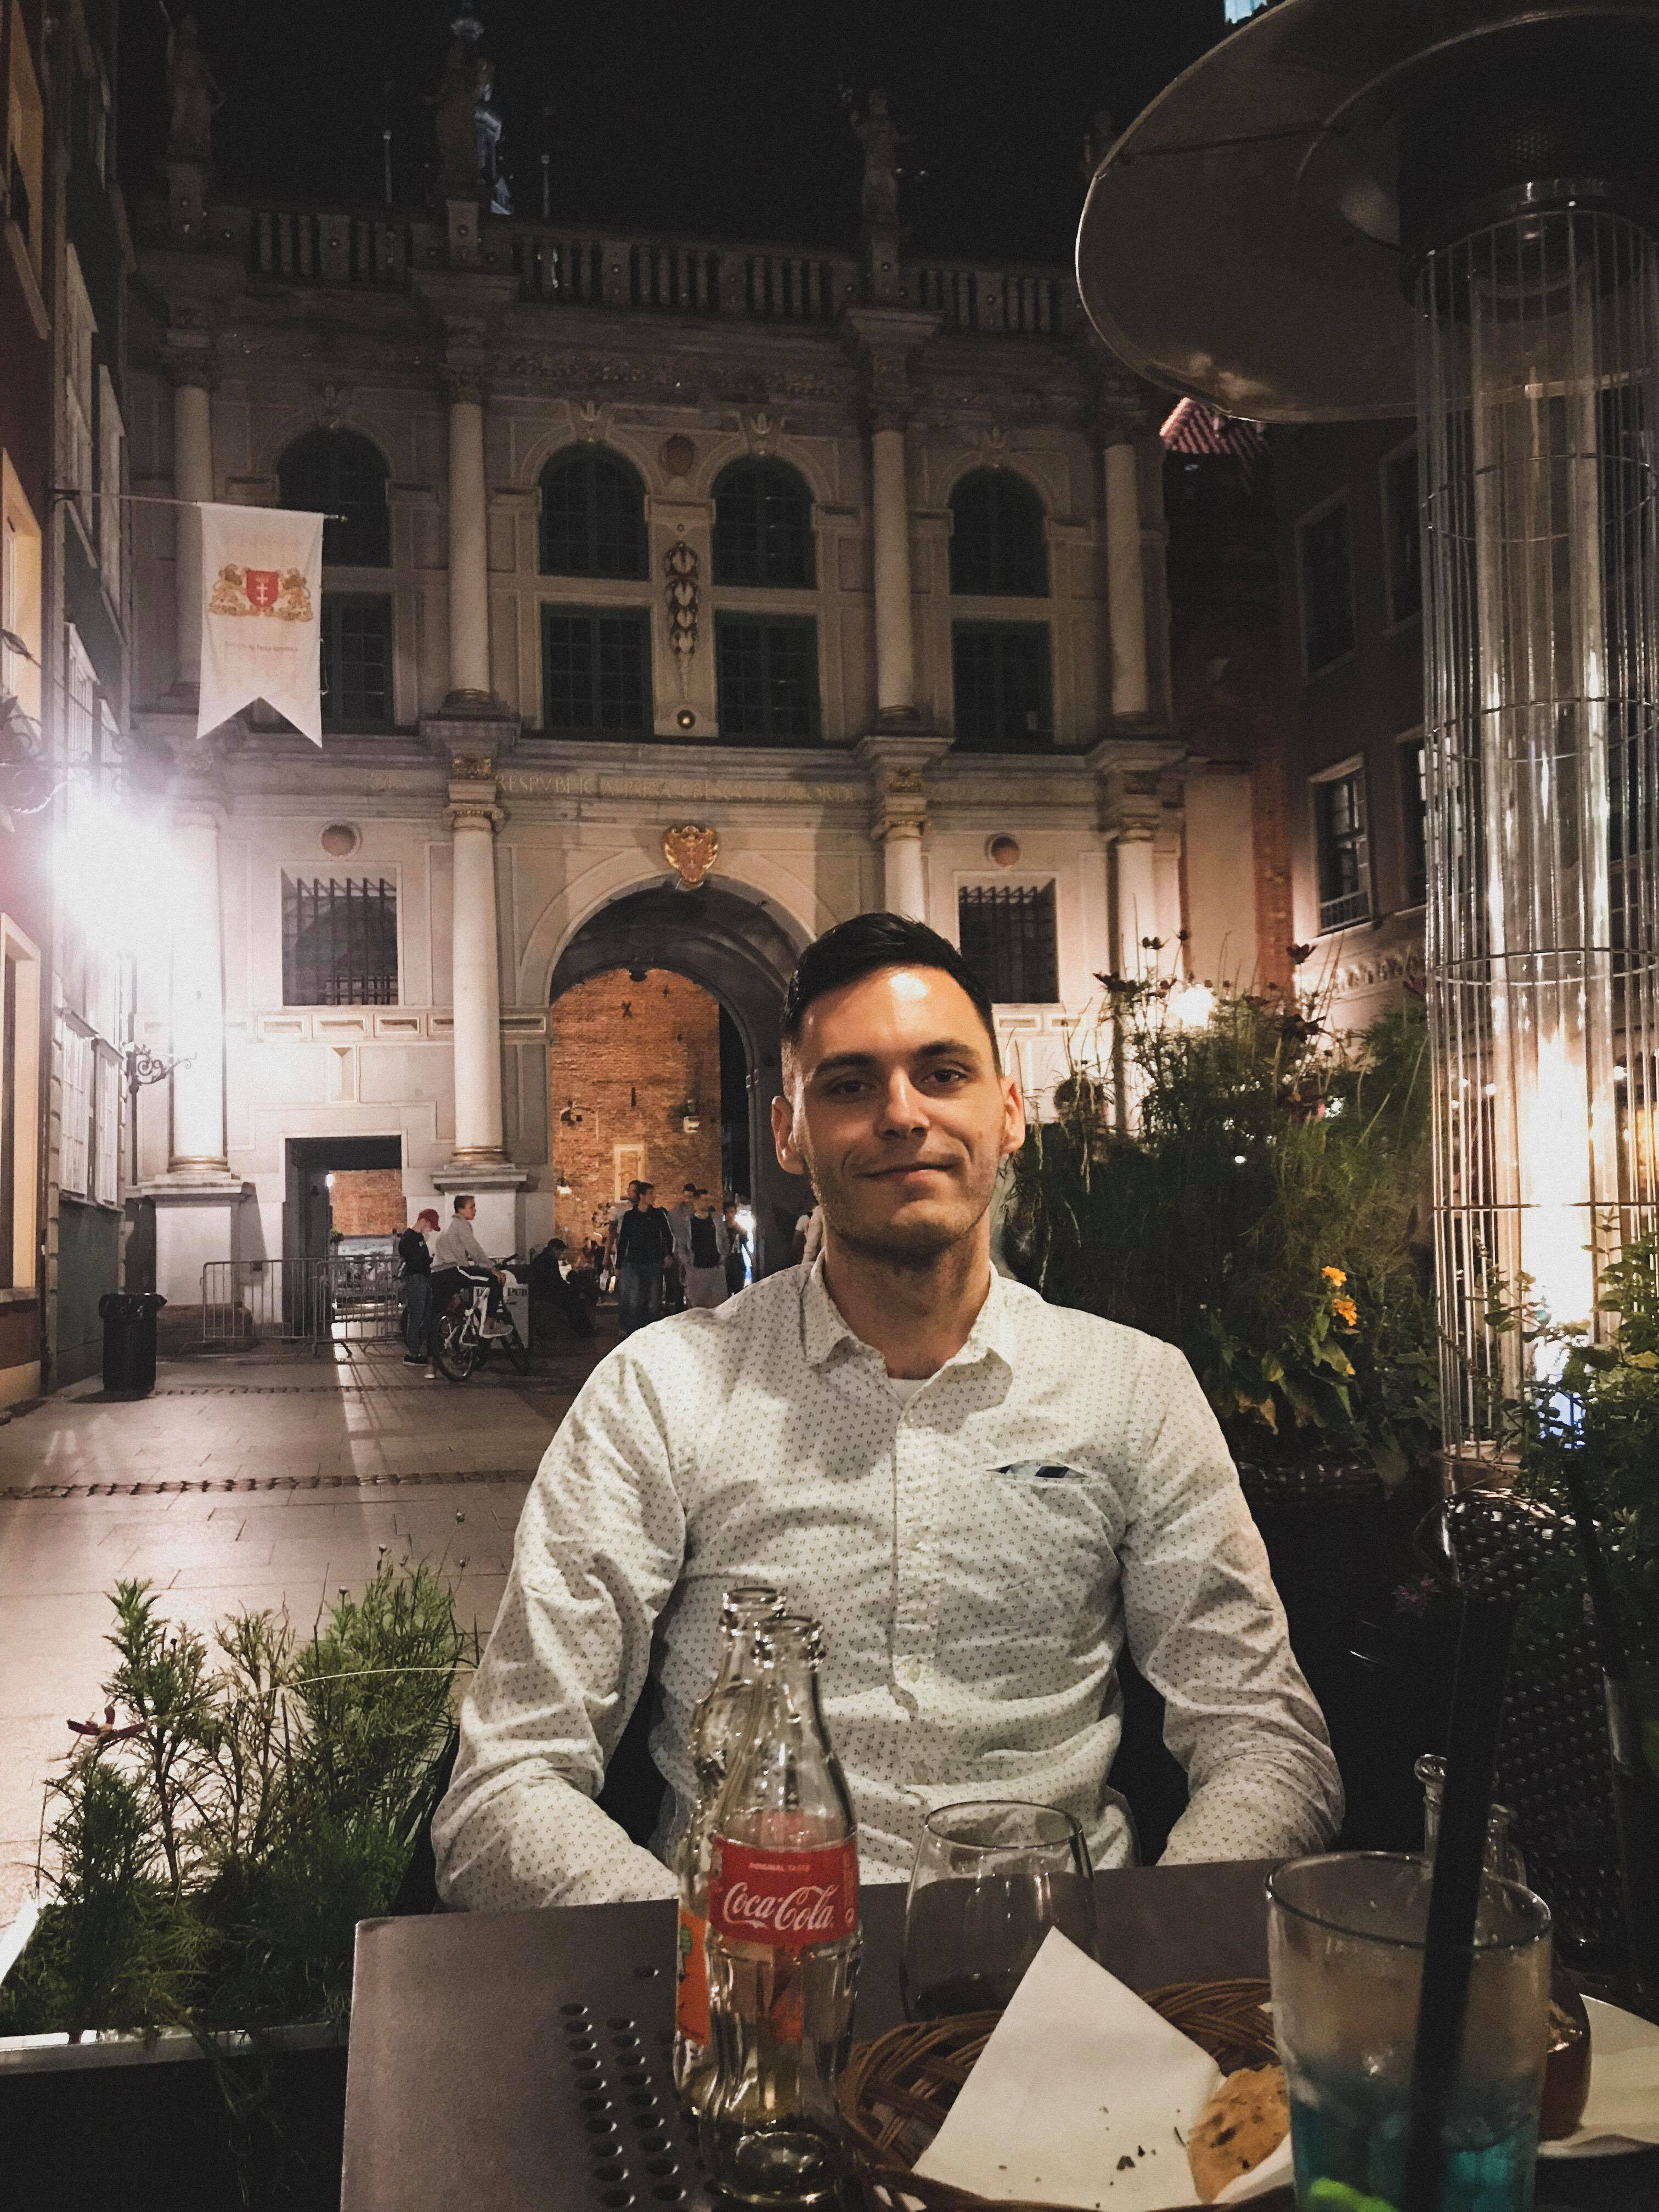
\includegraphics[width=0.30\textwidth]{pb}
%\end{wrapfigure}

\MyName{Lars Berge}
\MySlogan{Curriculum Vitae}

\sepspace

%%% Personal details
%%% ------------------------------------------------------------
\NewPart{Personlige opplysninger}{}

\PersonalEntry{Født}{Mai 7, 1996}
\PersonalEntry{Addresse}{Kringsjåvegen 39, Ålesund}
\PersonalEntry{Telefon}{45480990}
\PersonalEntry{Mail}{\url{bergelars96@gmail.com}}

%%% Education
%%% ------------------------------------------------------------
\NewPart{Utdanning}{}

\EducationEntry{Bachelor. Automatiseringsteknikk}{2017-2020}{NTNU i Ålesund}
{Ferdig våren 2020.
}
\sepspace

\EducationEntry{Automatiker lærling}{2015-2016}{Amatec AS}
{Fagprøve Bestått meget godt. \\
Årets Lærling i Opplæringskontoret for møbel, tre- og mekansik industri
}
\sepspace

\EducationEntry{VGS. Automatiseringsfaget}{2014-2015}{Sykkylven VGS}
{gjennomsnitt: 5,39 \\
Beste avgongselev Yrkesfagleg Utdanningsprogram.}
\sepspace

\EducationEntry{VGS. Automatisering}{2013-2014}{Sykkylven VGS}
{gjennomsnitt VG1 \& VG2: 5,47 \\
Beste avgongselev Yrkesfagleg Utdanningsprogram.}
\sepspace

\EducationEntry{VGS. Elektro}{2012-2013}{Sykkylven VGS}
{gjennomsnitt VG1 \& VG2: 5,47 }
\sepspace



%%% Work experience
%%% ------------------------------------------------------------
\NewPart{Erfaring}{}

\EducationEntry{Automatiker}{2018-}{Galavano AS, Sommer \& Tilkalling}
{Bygging av nytt lakkanlegg:
Montering av herdeovn
skriv her ka du gjor for greiff
Montering av kabelgater \& belysning
montering elektrisk utstyr
Trekking av kabel.}
\sepspace

\EducationEntry{Automatiker}{2017}{Amatec AS, Deltid}
{Tegning av EL-skjema i EPLAN \\
Bygging av styreskap \\
Programmering av PLS \\
Bygging av mekaniske konstruksjoner \\
Idriftsettelse av maskiner \& opplæring}
\sepsace

\EducationEntry{Arbeider}{2012-}{BB Montering AS, Deltid}
{Grunnarbeid, tilrettlegging, muring, forskaling, \\
snikkering, montering, måling
}
\sepsace

\EducationEntry{Heisvakt}{2015}{Strandafjellet skisenter AS, Deltid}
{Helg og kveld vinter 2015\\
Heisvakt ved alle typer skitrekk, blant annet stolheis og gondol
}
\sepsace

\EducationEntry{Renholdsarbeider}{Usikker}{Straumsheim glass \& fasade AS, Deltid}
{Rengjøring av produskjonområder og maskiner
}
\sepsace

%%% Skills
%%% ------------------------------------------------------------
\NewPart{Ferdigheter}{}

\SkillsEntry{Språk}{Norsk (morsmål)}
\SkillsEntry{}{English (fluent)}

\SkillsEntry{Programvare}
{\textsc{Matlab},
% \LaTeX, 
\textsc{Java}, 
\textsc{PLS}}
\SkillsEntry{Office}
{\textsc{Word},
\textsc{Excel}}



%%% Kurs
%%% ------------------------------------------------------------
\NewPart{Kurs}{}
\SkillsEntry{EMC-kurs}{Omron AS}


%%% Skuleinfo
%%% ------------------------------------------------------------
\NewPart{Emner bacheleor}{}
1.Semester \\
Matematikk sommerkurs R1 \& R2,	Fysikk TRES, Mikrokontrollere \\
Introduksjon til ingeniørfaget, Matematikk 1 \\
2.Semester \\
Elektronikk, Fysikk og kjemi, \\
Objektorientert programmering, Kommunikasjon og norsk, \\
3.Semester \\
Datakommunikasjon med nettverksprogrammering \\
Industrielle styresystemer, Matematikk 2A \\
4.Semester \\
Måleteknikk med statistikk, Signalbehandling, \\
Reguleringsteknikk \\
% Intelligente systemer \\
% Bildeanalyse \\
%Sanntids datateknikk \\





%%% References
%%% ------------------------------------------------------------
\NewPart{References}{}
Available upon request
\end{document}
